
\documentclass[numbertotal,toc,wide]{../bpslides}

\usepackage{blindtext}

\definecolor{green0}{rgb}{0,0.5,0}
\definecolor{red0}{rgb}{0.8,0,0}
\definecolor{blue0}{rgb}{0,0.2,0.8}
\definecolor{black0}{rgb}{0,0,0}
\definecolor{orange0}{rgb}{1,0.25,0}
\definecolor{magenta0}{cmyk}{0,1,0,0}
\definecolor{purple0}{rgb}{0.5,0,1}

%%%%%%%%%%%%%%%%%%%%%%%%

\title{Title of your presentation}

\subtitle{Subtitle of the presentation}

\author{Author 1\inst{1} \and Author 2\inst{2} \and Author 3\inst{3}}

\institute{\inst{1} Institution 1, \  \inst{2} Institution 2, \  \inst{3} Institution 3}

\conference{Conference/university hosting the talk}

\date{\today}

\disclaimer{The opinions and analyses in this paper are the responsibility of the authors and, therefore, do not necessarily coincide with those of their employers.}

\foot{Whatever you want to write}

%%%%%%%%%%%%%%%%%%%%%%%%

\begin{document}

\begin{frame}[plain]
	\titlepage
\end{frame}

\begin{frame}{Main options}\label{firstslide}
	\vspace{-0.3cm}
	\begin{center}\texttt{$\backslash$documentclass[\,\,\,\,options\,\,\,\,]\{bpslides\}}\end{center}\vspace{0.05cm}
	\begin{itemize}
		\item \texttt{numbering}: include slide numbers in the (right) footer
		\item \texttt{numbertotal}: include slide number and total number of slides in the (right) footer
		\item \texttt{toc}: table of contents at the beginning of each section and section title in the footer.\vs\\
		{\small\note{If sections are defined but this option is not selected, headings will show up in a separate slide at the beginning of each section and no section title will appear in the footer.}}
		\item \texttt{wide}: change the aspect ratio of the slides from 4:3 (default) to 16:9
		\item \texttt{color}: {\color{blue0}\texttt{blue}} \note{(default)}, {\color{green0}\texttt{green}}, {\color{red0}\texttt{red}}, {\color{orange0}\texttt{orange}}, {\color{black}\texttt{black}}, {\color{magenta0}\texttt{magenta}}, {\color{purple0}\texttt{purple}}\vs\\
		{\small\note{This option changes the main color of the slides, i.e., the color of titles, subtitles, blocks, buttons, etc.. The selected color is stored in \texttt{main}, so it can be used  with \texttt{\{$\backslash$color\{main\}...\}.}}}
		\item \texttt{font}: \texttt{sans} \note{(default)}, \texttt{helvetica}, \texttt{palatino}, \texttt{bookman}, \texttt{termes}, \texttt{adventor}
	\end{itemize}
	\vfill
\end{frame}

\section{Itemize and enumerate environments}

\subsection{Itemize environment}

\begin{frame}{Itemize}
Lorem ipsum dolor sit amet, consectetur adipiscing elit, sed do eiusmod tempor incididunt ut labore et dolore magna aliqua. 
	\begin{itemize}
		\item Lorem ipsum dolor sit amet, consectetur adipiscing elit, sed do eiusmod tempor incididunt ut labore et dolore magna aliqua.
		\begin{itemize}
			\item Lorem ipsum dolor sit amet, consectetur adipiscing elit, sed do eiusmod tempor incididunt ut labore et dolore magna aliqua.
			\begin{itemize}
				\item Lorem ipsum dolor sit amet, consectetur adipiscing elit, sed do eiusmod tempor incididunt ut labore et dolore magna aliqua.
			\end{itemize}
		\end{itemize}
		\item Lorem ipsum dolor sit amet, consectetur adipiscing elit, sed do eiusmod tempor incididunt ut labore et dolore magna aliqua.
	\end{itemize}
\end{frame}

\begin{frame}{Enumerate}{This is how a frame's subtitle looks like}
Lorem ipsum dolor sit amet, consectetur adipiscing elit, sed do eiusmod tempor incididunt ut labore et dolore magna aliqua. 
	\begin{enumerate}
		\item Lorem ipsum dolor sit amet, consectetur adipiscing elit, sed do eiusmod tempor incididunt ut labore et dolore magna aliqua.
		\begin{enumerate}
			\item Lorem ipsum dolor sit amet, consectetur adipiscing elit, sed do eiusmod tempor incididunt ut labore et dolore magna aliqua. 
			\begin{enumerate}
				\item Lorem ipsum dolor sit amet, consectetur adipiscing elit, sed do eiusmod tempor incididunt ut labore et dolore magna aliqua. 
			\end{enumerate}
		\end{enumerate}
		\item Lorem ipsum dolor sit amet, consectetur adipiscing elit, sed do eiusmod tempor incididunt ut labore et dolore magna aliqua. 
	\end{enumerate}
\end{frame}

\section{Blocks and buttons}

\begin{frame}{Blocks}
	\vfill
	\begin{block}{Example of a block}
		Lorem ipsum dolor sit amet, consectetur adipiscing elit, sed do eiusmod tempor incididunt ut labore et dolore magna aliqua. Ut enim ad minim veniam, quis nostrud exercitation ullamco laboris nisi ut aliquip ex ea commodo consequat.
	\end{block}
	\vfill
	\begin{center}
		\begin{minipage}{0.95\textwidth}
			\texttt{$\backslash$begin\{block\}\{Example of a block\}}\vs\par
			Lorem ipsum dolor sit amet, consectetur adipiscing elit, sed do eiusmod tempor incididunt ut labore et dolore magna aliqua. Ut enim ad minim veniam, quis nostrud exercitation ullamco laboris nisi ut aliquip ex ea commodo consequat.\vs\par
			\texttt{$\backslash$end\{block\}}
		\end{minipage}
	\end{center}
	\vfill
\end{frame}


\begin{frame}{Buttons}
	\vfill
	\begin{itemize}
		\item Lorem ipsum dolor sit amet, consectetur adipiscing elit, sed do eiusmod tempor incididunt ut labore et dolore magna aliqua. Ut enim ad minim veniam, quis nostrud exercitation ullamco laboris nisi ut aliquip ex ea commodo consequat.
		\item Lorem ipsum dolor sit amet, consectetur adipiscing elit, sed do eiusmod tempor incididunt ut labore et dolore magna aliqua. Ut enim ad minim veniam, quis nostrud exercitation ullamco laboris nisi ut aliquip ex ea commodo consequat.
	\end{itemize}
	\vfill
	\hfill
	\texttt{$\backslash$button\{firstslide\}\{back to first slide\}} 
	$\so$
	\button{firstslide}{back to first slide}
\end{frame}

\section{Tables and figures}

\begin{frame}{Tables}
	\begin{table}
		\centering
		\caption{Heading of the table}
		\begin{tabular}{cccc} \toprule
		& Mean & Median & Std Desvi.\\ \midrule
		Variable 1 & $1150$ & 900 & 235 \\ 
		Variable 2 & $430$ & 300 & 57 \\ 
		Variable 3 & $367$ & 210 & 113 \\ \bottomrule
		\end{tabular}
	\end{table}
\end{frame}

\begin{frame}{Figures}
	\begin{figure}
		\centering
		\caption{Heading of the figure}
		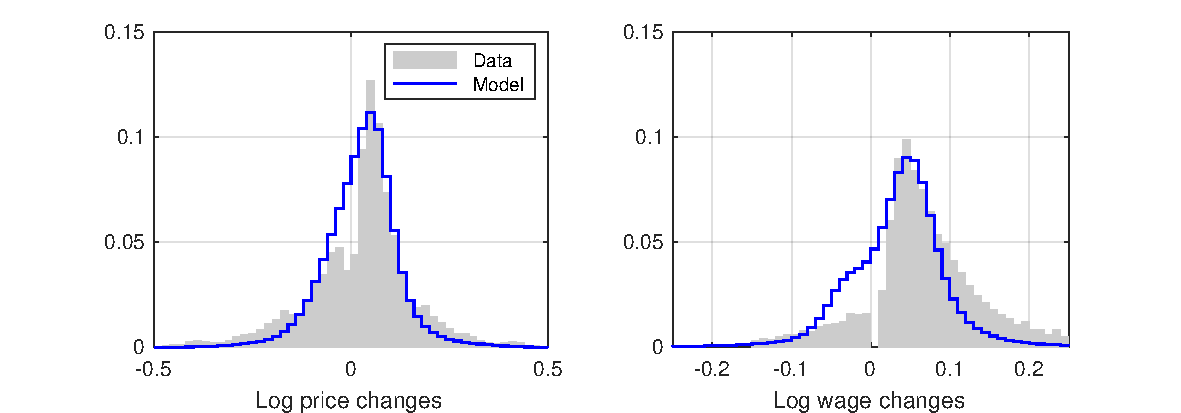
\includegraphics[width=0.9\textwidth]{figure.pdf}
		\vs\vs\par
		\begin{minipage}{0.75\textwidth}\scriptsize%
		Source: Figure 2 in \paper{Costain, Nakov, and Petit}{2022}
		\end{minipage}
	\end{figure}
\end{frame}

\section{New commands}

\begin{frame}{New commands}{In preambule}
	\begin{itemize}
		\item \texttt{$\backslash$foot$\{$What ever you want to write$\}$} 
		\begin{itemize}
			\item[] displays ``Whatever you want to write'' in the bottom-left corner
		\end{itemize}
		\item \texttt{$\backslash$conference$\{$the place$\}$}
		\begin{itemize}
			\item[] displays the institution hosting the talk in the title page
		\end{itemize}
		\item \texttt{$\backslash$disclaimer$\{$something$\}$} 
		\begin{itemize}
			\item[] displays a footnote in the title page with a disclaimer
		\end{itemize}
	\end{itemize}
\end{frame}

% \begin{frame}{New commands}{In main text}
% 	\begin{itemize}
% 		\item \texttt{$\backslash$paper$\{$Author$\}\{$Year$\}$} displays \paper{Author}{Year}
% 		\begin{itemize}
% 			\item[] Code: \texttt{I use the slides in $\backslash$paper$\{$Petit$\}\{$2025$\}$, the best slides ever.}
% 			\item[] Result: I use the slides in \paper{Petit}{2025}, the best slides ever.
% 		\end{itemize}
% 		\item \texttt{$\backslash$paperalt$\{$Author$\}\{$Year$\}$} displays \paperalt{Author}{Year}
% 		\item \texttt{$\backslash$alert$\{$Lorem ipsum$\}$} displays \alert{Lorem ipsum}
% 		\item \texttt{$\backslash$note$\{$Lorem ipsum$\}$} displays \note{Lorem ipsum}
% 		\item \texttt{$\backslash$under$\{$Lorem ipsum$\}$} displays \under{Lorem ipsum}
% 		\item \texttt{$\backslash$vs}: equivalent to \texttt{$\backslash$vspace$\{$0.1cm$\}$}
% 		\item \texttt{$\backslash$hs}: equivalent to \texttt{$\backslash$hspace$\{$0.1cm$\}$}
% 		\item \texttt{$\backslash$boxed$\{$Lorem ipsum$\}$} displays\vs\vs\\ \boxed{Lorem ipsum}
% 	\end{itemize}
% \end{frame}

\begin{frame}{New commands}{In main text}
	\begin{center}
		\def\arraystretch{1.5}%
		\begin{tabular}{ll} \toprule
			Code & Result \\ \midrule
			\texttt{$\backslash$paper$\{$Author$\}\{$Year$\}$} & \paper{Author}{Year} \\
			\texttt{$\backslash$paperalt$\{$Author$\}\{$Year$\}$} &\paperalt{Author}{Year} \\
			\texttt{$\backslash$alert$\{$Lorem ipsum$\}$} & \alert{Lorem ipsum} \\
			\texttt{$\backslash$note$\{$Lorem ipsum$\}$} & \note{Lorem ipsum} \\
			\texttt{$\backslash$under$\{$Lorem ipsum$\}$} & \under{Lorem ipsum} \\
			% \texttt{$\backslash$vs} & equivalent to \texttt{$\backslash$vspace$\{$0.1cm$\}$} \\
			% \texttt{$\backslash$hs} & equivalent to \texttt{$\backslash$hspace$\{$0.1cm$\}$} \\
			\texttt{$\backslash$boxed$\{$Lorem ipsum$\}$} &  \boxed{Lorem ipsum} \\
			\bottomrule
		\end{tabular}
	\end{center}
	\vfill
	% \begin{itemize}
	% 	\item \texttt{$\backslash$paper$\{$Author$\}\{$Year$\}$} $\so$ \paper{Author}{Year}
	% 	\item \texttt{$\backslash$paperalt$\{$Author$\}\{$Year$\}$} $\so$ \paperalt{Author}{Year}
	% 	\item \texttt{$\backslash$alert$\{$Lorem ipsum$\}$} $\so$ \alert{Lorem ipsum}
	% 	\item \texttt{$\backslash$note$\{$Lorem ipsum$\}$} $\so$ \note{Lorem ipsum}
	% 	\item \texttt{$\backslash$under$\{$Lorem ipsum$\}$} $\so$ \under{Lorem ipsum}
	% 	\item \texttt{$\backslash$vs}: equivalent to \texttt{$\backslash$vspace$\{$0.1cm$\}$}
	% 	\item \texttt{$\backslash$hs}: equivalent to \texttt{$\backslash$hspace$\{$0.1cm$\}$}
	% 	\item \texttt{$\backslash$boxed$\{$Lorem ipsum$\}$} $\so$  \boxed{Lorem ipsum}
	% \end{itemize}
\end{frame}

\begin{frame}{New commands}{In math mode}
	\begin{itemize}
		\item \texttt{$\backslash$mathpause}: addapted version of the standard \texttt{$\backslash$pause} command to avoid the extra vertical space that \texttt{$\backslash$pause} adds in math mode.
		\item \texttt{$\backslash$so}: displays a long rigth arrow ($\longrightarrow$) in the main color.\vs\\\note{This commenad needs to be used in math mode.}
		\item \texttt{$\backslash$eqboxed$\{$x = 0$\}$} displays $x=0$ in a box.
	\end{itemize}\vs\vs\vs
	Example: \texttt{\$\$$\backslash$llave$\{$x = exp(1)$\}$$\{$An equation$\}$  $\backslash$mathpause $\backslash$so $\backslash$eqboxed$\{$x = 0$\}$\$\$}
	$$\llave{x = \exp(1)}{An equation} \mathpause \so \eqboxed{x=0}$$
	\vfill
\end{frame}

\begin{frame}[plain]{}
	\begin{center}{\Large
		\alert{Comments and suggestions are very welcome}\vs\vs\vs\vs\vs\vs\par \href{mailto:bpetit@cunef.edu}{bpetit [at] cunef.edu}
		}
	\end{center}
\end{frame}

\end{document}
